%%%%%%%%%%%%%%%%%%%%%%%%%%%%%%%%%%%%%%
% LaTeX poster template
% Created by Nathaniel Johnston
% August 2009
% http://www.nathanieljohnston.com/index.php/2009/08/latex-poster-template/
%%%%%%%%%%%%%%%%%%%%%%%%%%%%%%%%%%%%%%

\documentclass[final]{beamer}
\usepackage[scale=1.24]{beamerposter}
\usepackage{graphicx}			% allows us to import images

%-----------------------------------------------------------
% Define the column width and poster size
% To set effective sepwid, onecolwid and twocolwid values, first choose how many columns you want and how much separation you want between columns
% The separation I chose is 0.024 and I want 4 columns
% Then set onecolwid to be (1-(4+1)*0.024)/4 = 0.22
% Set twocolwid to be 2*onecolwid + sepwid = 0.464
%-----------------------------------------------------------

\newlength{\sepwid}
\newlength{\onecolwid}
\newlength{\twocolwid}
\newlength{\threecolwid}
\setlength{\paperwidth}{48in}
\setlength{\paperheight}{36in}
\setlength{\sepwid}{0.03\paperwidth}
\setlength{\onecolwid}{0.2125\paperwidth}
\setlength{\twocolwid}{0.455\paperwidth}
\setlength{\threecolwid}{0.708\paperwidth}
\setlength{\topmargin}{-0.5in}
\usetheme{confposter}

%-----------------------------------------------------------
% Define colours (see beamerthemeconfposter.sty to change these colour definitions)
%-----------------------------------------------------------

\setbeamercolor{block title}{fg=ngreen,bg=white}
\setbeamercolor{block body}{fg=black,bg=white}
\setbeamercolor{block alerted title}{fg=white,bg=dblue!70}
\setbeamercolor{block alerted body}{fg=black,bg=dblue!10}
\setbeamertemplate{caption}[numbered]

%-----------------------------------------------------------
% Name and authors of poster/paper/research
%-----------------------------------------------------------

\title{PHI Redaction for Neuroimagery}
\author{Nakeisha Schimke\texorpdfstring{$^1$}{}, Alex Barclay\texorpdfstring{$^{1,2}$}{}, Peter Gehres\texorpdfstring{$^{1,2}$}{}, and John Hale\texorpdfstring{$^1$}{}}
\institute{\texorpdfstring{$^1$}{}Institute for Bioinformatics and Computational Biology, University of Tulsa \hspace{2in} \texorpdfstring{$^2$}{}Laureate Institute for Brain Research, Tulsa, Oklahoma}

%-----------------------------------------------------------
% Start the poster itself
%-----------------------------------------------------------
% The \rmfamily command is used frequently throughout the poster to force a serif font to be used for the body text
% Serif font is better for small text, sans-serif font is better for headers (for readability reasons)
%-----------------------------------------------------------

\begin{document}
\begin{frame}[t]
  \begin{columns}[t]												% the [t] option aligns the column's content at the top
    \begin{column}{\sepwid}\end{column}			% empty spacer column
    \begin{column}{\onecolwid}
% BEGIN OBJECTIVES BLOCK
      \begin{block}{Objectives}
%        \rmfamily{In order for your poster to compile properly, up-to-date versions of the following packages are required:
%        \vskip1ex
%        \begin{itemize}
%          \item latexbeamer
%          \item pgf (Tikz)
%          \item beamerposter
%        \end{itemize}
%        \vskip1ex
%        All of those packages are contained in both the MikTeX and the TexLive distribution of LaTeX.}
				 \rmfamily{
The potential for large scale collaboration and data sharing is seriously undermined by concerns over the management and handling of PII in neuroimagery data sets. 
%HIPAA and HITECH rules mandate substantial measures for the preservation of subject privacy, and for the researcher, the management of information privacy is a burdensome task. The potential for sharing and meta analysis of neuroimagery in research goes unfulfilled for two reasons: (1) sanitization is hampered by the lack of tools to systematically expunge PHI from DICOM images, and (2) an established workflow to integrate sanitization into the data sharing process remains conspicuously absent.
We address this problem by augmenting XNAT with a toolset and integrated workflow for pseudonymous redaction of PII in DICOM image files. 
The approach adopted by this effort gives researchers the maximum power and flexibility in sharing neuroimagery datasets while transparently coping with PII considerations in a standardized data curation process.
%\vskip2ex

%To satisfy HIPAA requirements while maintaining ease of use, we offer an automated approach to redacting patient data for use with the eXtensible Neuroimage Archive Toolkit (XNAT) as a repository, folding neatly within existing XNAT operational workflows and processes.

}
			\end{block}
			\vskip2ex
% END OBJECTIVES BLOCK
      
      
% BEGIN BLOCK: REDACTION
      \begin{block}{Neuroimage Data Stack}
        \rmfamily{
To ensure comprehensive redaction, we have logically deconstructed neuroimage data sets in a layered approach at the hardware, operating system, and data analysis levels.
At the simplest and lowest level on the stack, the raw neuroimage data exists on physical storage media (eg. hard drives) in a binary form as a stream of data.  
At the file system level, the neuroimage is represented as a file pointer to an address space on the physical disk, along with associated metadata.
The DICOM file format is the middle layer, containing both metadata and pixel data in a single file.
The image pixel data can be encapsulated for compression purposes, and the logical layer is the resulting neuroimage.
        }
%        \begin{semiverbatim}
%          {\color{red}\\begin}\{{\color{blue}block}\}\{Title\}\newline
%          \hskip1ex.......\newline
%          {\color{red}\\end}\{{\color{blue}block}\}
%        \end{semiverbatim}}
      \end{block}
      \vskip2ex
% END BLOCK: REDACTION      

% BEGIN BLOCK: DICOM
      \begin{block}{DICOM Redaction}
        \rmfamily{
This project focuses on the DICOM layer, removing PII metadata from stored images.
This tool is an extension of XNAT to seamlessly integrate redaction into the natural analysis and archive process, lessening the burden of data management on the end user by providing sanitization and verification along with persistent pseudonymous identifiers.
}
      \end{block}
      \vskip2ex
% END BLOCK: DICOM

\end{column}
%
\begin{column}{\sepwid}\end{column}
\begin{column}{\onecolwid}
% BEGIN BLOCK: WORKFLOW
      \begin{block}{Workflow}
%        \rmfamily{The standard block environment looks like this. It has justified text and a green title with an underline. You can create one like so:
%        \begin{semiverbatim}
%          {\color{red}\\begin}\{{\color{blue}block}\}\{Title\}\newline
%          \hskip1ex.......\newline
%          {\color{red}\\end}\{{\color{blue}block}\}
%        \end{semiverbatim}}
\rmfamily{
The primary workflow is based on the XNAT workflow, so that to the researcher, it remains unchanged, as shown in Figure~\ref{fig:userworkflow}.
The process begins at acquisition and is stored according to the local institution's policy.
Once it is released from quarantine, the redaction process can be invoked by the user.
This produces a new sanitized data set with pseudonymous identifiers that is sent to the quarantined pre-archive area, mandating a second sanity check before releasing it to the XNAT archive.
Once it enters the XNAT archive, it is treated as normal data and is available for analysis without modifications to XNAT itself.
This new data set contains privacy mapped identifiers available only to a subset of users and can be publicly shared.
%It may be desirable to retain some of the original embedded subject data (such as age, weight, etc) in the redacted data set; in this case, it is up to the end user to verify that the

\vskip2ex

A logical view of the data is shown in Figure~\ref{fig:logicalworkflow}.
XNAT invokes our external redaction engine, which makes a sanitizes a copy of the data and stores the PII in the privacy map.
The redacted data set is fed back into XNAT.
The privacy map is not made available to the end user but is accessible to administrators through a command-line tool.

}
\end{block}

\vskip2ex

\begin{figure}
\begin{center}
\includegraphics[scale=1.0]{workflow_pipeline.png}
\caption{Neuroimage data redaction workflow, as experienced by the end user.}
\label{fig:userworkflow}
\end{center}
\end{figure}

\vskip2ex

\begin{figure}
\begin{center}
\includegraphics[scale=1.0]{data_workflow.png}
\caption{XNAT and redaction logical workflow, with modifications in bold.}
\label{fig:logicalworkflow}
\end{center}
\end{figure}

\end{column}
\begin{column}{\sepwid}\end{column}
\begin{column}{\onecolwid}      
%      \vskip2ex
% END BLOCK: WORKFLOW
\begin{figure}
\begin{center}
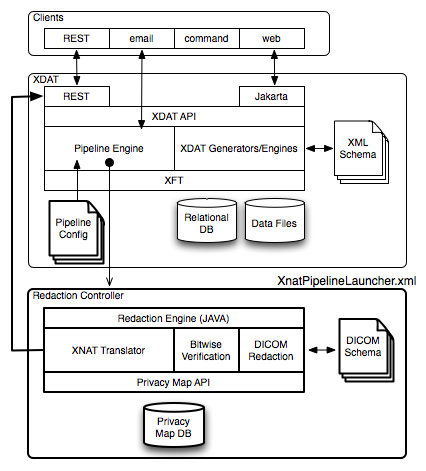
\includegraphics[scale=1.5 ]{architecture_pipeline.png}
\caption{Modified architecture diagram.}
\label{fig:architecture}
\end{center}
\end{figure}
%\begin{column}{\twocolwid}
%\begin{block}
%\begin{figure}
%\begin{center}
%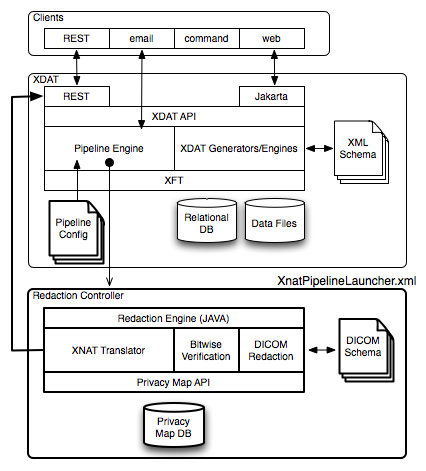
\includegraphics[scale=1.5]{architecture_pipeline.png}
%\caption{Modified architecture diagram.}
%\label{fig:architecture}
%\end{center}
%\end{figure}
%\end{block}
%\begin{columns}[t,totalwidth=\twocolwid]
%\end{block}
%\end{column}
%\begin{column}{\sepwid}\end{column}
%\begin{column}{\onecolwid}
% BEGIN BLOCK: ARCHITECTURE
      \begin{block}{Architecture}
      \rmfamily{
There are three primary logical components: (1) the redaction engine, (2) the privacy map, and (3) the 	XNAT translator.  
The redaction engine and privacy map integrate into the XNAT pipeline facility, enabling an XNAT-aware redaction process capable of providing feedback, status tracking and debugging features within XNAT.

\vskip2ex

The redaction engine serves as an expandable entry point and contains both DICOM image redaction procedures and a low-level bitwise verification mechanism to fully remove embedded PII. The privacy map is an encrypted database containing the link between the original images and their redacted counterparts, accessible only by an API to ensure the integrity of the databases by exposing a non-harmful subset of commands to the redaction engine. It provides consistency between research subjects of the redacted ID to subject PII, preventing statistical skew due to data duplication. The XNAT translator creates new XNAT identifiers and transmits redacted data in a format recognizable by XNAT.
%
%\vskip2ex
%
%The DICOM redaction component is based on detailed knowledge of the DICOM format and the conformance statements provided by the major MRI vendors.
%A list of name:value pairs are extracted from the DICOM file itself, and these tuples are remapped to anonymized identifiers through the use of DICOM image translation schemas.
%The shipping configuration is tailored to HIPAA compliance, though this is fully customizable.
}
%        \rmfamily{The standard block environment looks like this. It has justified text and a green title with an underline. You can create one like so:
%        \begin{semiverbatim}
%          {\color{red}\\begin}\{{\color{blue}block}\}\{Title\}\newline
%          \hskip1ex.......\newline
%          {\color{red}\\end}\{{\color{blue}block}\}
%        \end{semiverbatim}}
      \end{block}
      \vskip2ex
% END BLOCK: ARCHITECTURE 
\end{column}

\begin{column}{\sepwid}\end{column}
\begin{column}{\onecolwid}

% BEGIN BLOCK: ADVANTAGES
      \begin{block}{Advantages}
      \rmfamily{
The privacy map provides a mechanism for linking and managing subjects across institutional boundaries by removing PII and creating pseudonymous identifiers.
This transparently maintains mapped subject identifiers throughout a study and ensures the persistence of the redacted identifier over multiple imaging sessions.
As part of the XNAT processing pipeline, we leverage the existing framework and interface of XNAT, and redaction becomes a natural part of the existing workflow.
The redaction process is forensically verifiable to ensure confidentially of subject data.
This technique is accepted for handling digital evidence, providing researchers legally accepted protection and assurance that shared subject data does not fall under the breach notification requirements of HIPAA/HITECH.
}
%        \rmfamily{The standard block environment looks like this. It has justified text and a green title with an underline. You can create one like so:
%        \begin{semiverbatim}
%          {\color{red}\\begin}\{{\color{blue}block}\}\{Title\}\newline
%          \hskip1ex.......\newline
%          {\color{red}\\end}\{{\color{blue}block}\}
%        \end{semiverbatim}}
      \end{block}
      \vskip2ex
% END BLOCK: ADVANTAGES


% BEGIN BLOCK: POTENTIAL CHALLENGES
      \begin{block}{Future Work}
      	 \rmfamily{This effort will be expanded to integrate a comprehensive plan for neuroimage redaction.  
We plan to include mechanisms for redaction at the hard drive and file systems, as well as a defacing technique for structural images.}
%        \rmfamily{The standard block environment looks like this. It has justified text and a green title with an underline. You can create one like so:
%        \begin{semiverbatim}
%          {\color{red}\\begin}\{{\color{blue}block}\}\{Title\}\newline
%          \hskip1ex.......\newline
%          {\color{red}\\end}\{{\color{blue}block}\}
%        \end{semiverbatim}}
      \end{block}
      \vskip2ex
% END BLOCK: POTENTIAL CHALLENGES  

%      \begin{alertblock}{An ``Alert'' Block}
%        \rmfamily{The ``alert'' block environment looks like this. It also has justified text, but it has a border and a light background to make it stand out. You can create one like so:
%        \begin{semiverbatim}
%          {\color{red}\\begin}\{{\color{blue}alertblock}\}\{Title\}\newline
%          \hskip1ex.......\newline
%          {\color{red}\\end}\{{\color{blue}alertblock}\}
%        \end{semiverbatim}}
%      \end{alertblock}
%    \end{column}

%    \begin{column}{\sepwid}\end{column}			% empty spacer column
%    \begin{column}{\threecolwid}					  % create a three-column-wide column and then we will split it up later
%      \begin{block}{Altering Column Spans}
%        \rmfamily{You can make columns that span multiple other columns relatively easily. Lengths are defined in the template that make columns look normal-ish if you want to use a four-column layout like this poster. If you want to use a different number of columns, you will have to modify those lengths accordingly at the top of the poster.tex file.
%        
%        In particular, near the top of the TeX file you will see lines that look like:
%        \begin{semiverbatim}
%          \hskip1ex\\setlength\{\\sepwid\}\{0.024\\paperwidth\}
%          
%          \hskip1ex\\setlength\{\\onecolwid\}\{0.22\\paperwidth\}
%          
%          \hskip1ex\\setlength\{\\twocolwid\}\{0.464\\paperwidth\}
%          
%          \hskip1ex\\setlength\{\\threecolwid\}\{0.708\\paperwidth\}
%        \end{semiverbatim}}
%        
%        Set ``sepwid'' to be some small length somewhere near 0.025 (this is the space between columns). Then if $n$ is the number of columns you want, you should set
%        \begin{align*}
%          \text{onecolwid} & = \frac{1}{n}(1-(n+1)\times\text{sepwid}), \\
%          \text{twocolwid} & = 2\times\text{onecolwid} + \text{sepwid}, \\
%          \text{threecolwid} & = 3\times\text{onecolwid} + 2\times\text{sepwid}.
%        \end{align*}
%      \end{block}
%      \begin{columns}[t,totalwidth=\threecolwid]	% split up that three-column-wide column
%        \begin{column}{\onecolwid}
%          \setbeamercolor{block title}{fg=red,bg=white}%frame color
%          \setbeamercolor{block body}{fg=black,bg=white}%body color
%          \begin{block}{Block Colours}
%            \rmfamily{For the standard blocks there are two colours; one for the title and one for the block body:\\
%            \begin{semiverbatim}
%              {\color{red}\\setbeamercolor}\{block title\}\newline \{fg=red,bg=white\}
%            \end{semiverbatim}
%            \begin{semiverbatim}
%              {\color{red}\\setbeamercolor}\{block  body\}\newline \{fg=black,bg=white\}
%            \end{semiverbatim}
%            The \emph{fg} colour sets the text colour and \emph{bg} sets the background colour.
%            For the normal blocks it makes no sense to use a background colour other than white. You \emph{can} change it, but it will look weird!}
%          \end{block}
%        \end{column}
%        \begin{column}{\onecolwid}
%          \setbeamercolor{block alerted title}{fg=black,bg=norange}	% frame color
%          \setbeamercolor{block alerted body}{fg=black,bg=white}		% body color
%          \begin{alertblock}{Alert Block Colours}
%            \rmfamily{You can similarly modify the colours for alert blocks (but try not to overdo it):\\
%            \begin{semiverbatim}
%              {\color{red}\\setbeamercolor}\{block title\}\newline \{fg=black,bg=norange\}
%            \end{semiverbatim}
%            \begin{semiverbatim}
%              {\color{red}\\setbeamercolor}\{block  body\}\newline \{fg=black,bg=white\}
%            \end{semiverbatim}}
%          \end{alertblock}        
%        \end{column}
%        \begin{column}{\onecolwid}
          \begin{block}{References}
            \small{\rmfamily{\begin{thebibliography}{99}
		        \bibitem{xnat} {D.~W. Marcus, T. Olsen, M. Ramaratnam, and R.~L. Buckner, Neuroinformatics, \textbf{5(1)} (2006), 11-34.}
		        \bibitem{nrg} {NRG, Washington Univ. in St. Louis, Pipeline quick tutorial (2009).}
						\bibitem{hipaa} {E. McCallister, T. Grance, and K. Scarfone, NIST Special Publication 800-122 (draft) (2009).}
						\bibitem{dicom} {NEMA, Digital Imaging and Communications in Medicine (2008).}
						\bibitem{redaction} {A. Barclay, N. Schimke, and J. Hale, USENIX Security (2009).}
%						\bibitem{loni}{S.~C. Neu, D.~J. Valentino, and A.~W. Toga, Neuroimage, \textbf{24} (2005), 1170-1179.}
		        \end{thebibliography}}}
			      \vspace{0.75in}
		      \end{block}
		      \begin{block}{Acknowledgments}
		      We gratefully acknowledge support from the William K. Warren Foundation.
		      \end{block}
%        \end{column}
%      \end{columns}
      \vskip2ex
    \end{column}
  \begin{column}{\sepwid}\end{column}			% empty spacer column
 \end{columns}
\end{frame}
\end{document}
